% Shared standalone design for the editable figure reconstructions.
\documentclass[tikz,border=5pt,10pt]{standalone}
\usepackage[T1]{fontenc}
\usepackage[utf8]{inputenc}
\usepackage{newpxtext,newpxmath}
\usepackage[scaled=.94]{sourcesanspro}
\usepackage{pgfplots}
\pgfplotsset{compat=1.18}
\usetikzlibrary{arrows.meta,calc,positioning,decorations.pathreplacing,
  decorations.markings,patterns,matrix,shapes.geometric,fit,backgrounds,
  intersections,angles,quotes}
\definecolor{ink}{HTML}{203746}
\definecolor{accent}{HTML}{146C78}
\definecolor{muted}{HTML}{667780}
\definecolor{signalred}{HTML}{B94B44}
\color{ink}
\tikzset{>=Latex,line width=.8pt,
  every node/.style={font=\small},
  axis/.style={->,draw=muted,line width=.5pt},
  guide/.style={draw=muted,dashed,line width=.45pt},
  curve/.style={draw=accent,line width=1pt},
  marker/.style={circle,fill=accent,inner sep=1.5pt},
  labelbox/.style={fill=white,inner sep=2pt}}

\begin{document}
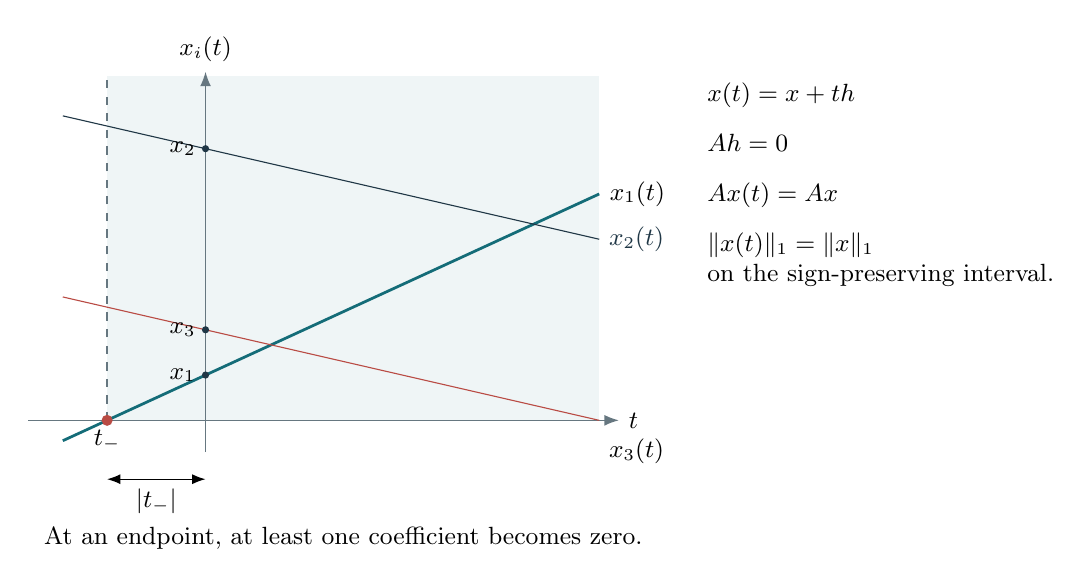
\begin{tikzpicture}[x=1.25cm,y=1.15cm]
\path[fill=accent!7](-1,0)rectangle(4,3.8);
\draw[axis](-1.8,0)--(4.2,0)node[right]{$t$};\draw[axis](0,-.35)--(0,3.85)node[above]{$x_i(t)$};
\draw[curve](-1.45,-.225)--(4,2.5)node[right]{$x_1(t)$};
\draw[ink](-1.45,3.3625)--(4,2)node[right]{$x_2(t)$};
\draw[signalred](-1.45,1.3625)--(4,0);\node[below right]at(4,-.1){$x_3(t)$};
\foreach \v/\lab in {.5/1,3/2,1/3}{\fill[ink](0,\v)circle(1.3pt);\node[left]at(0,\v){$x_\lab$};}
\draw[guide](-1,0)--(-1,3.8);\fill[signalred](-1,0)circle(2pt);\node[below]at(-1,0){$t_-$};
\draw[<->](-1,-.65)--(0,-.65)node[midway,below]{$|t_-|$};
\node[anchor=west,align=left]at(5,2.6){$x(t)=x+t h$\\[7pt]$Ah=0$\\[7pt]$Ax(t)=Ax$\\[7pt]$\|x(t)\|_1=\|x\|_1$\\on the sign-preserving interval.};
\node[align=center]at(1.4,-1.3){At an endpoint, at least one coefficient becomes zero.};
\end{tikzpicture}
\end{document}
